\documentclass{beamer}
%Opción para que no se muestre el índice completo en la izquierda de las diapositivas
\usetheme[ocultarotrassubsecciones]{UCLM}

% IDIOMA ESPAÑOL Y TILDES Y EÑES
\usepackage[utf8]{inputenc}
\usepackage[spanish, es-tabla]{babel}
\usepackage{graphicx}
\usepackage{multirow}
\usepackage{subfigure}
\usepackage{natbib}
\usepackage{appendix}
\usepackage[formats]{listings}
\usepackage{longtable}


\usepackage[utf8]{inputenc}
\usepackage{url}
 %\usepackage{graphicx} % Allows including images
\usepackage{booktabs} % Allows the use of \toprule, \midrule and \bottomrule in tables



\usepackage{xcolor}
\usepackage{textcomp}


\usepackage{courier}

% Definicion general para el código en todos los lenguajes
\lstset{
	%frame=single,
	breaklines=true,
	showstringspaces=false,
	postbreak=\raisebox{0ex}[0ex][0ex]{\ensuremath{\color{red}\hookrightarrow\space}},
	framexleftmargin=10mm,
}

% Default fixed font does not support bold face
%\DeclareFixedFont{\ttb}{T1}{txtt}{bx}{n}{12} % for bold
%\DeclareFixedFont{\ttm}{T1}{txtt}{m}{n}{12}  % for normal

% Definición de colotes
\usepackage{color}
\definecolor{deepblue}{rgb}{0,0,0.5}
\definecolor{deepred}{rgb}{0.6,0,0}
\definecolor{deepgreen}{rgb}{0,0.5,0}


% Estilo para Python
\newcommand\pythonstyle{\lstset{
		language=Python,
		%basicstyle=\ttm,
		otherkeywords={self},             % Add keywords here
		%keywordstyle=\ttb\color{deepblue},
		keywordstyle=\color{deepblue},
		emph={MyClass,__init__},          % Custom highlighting
		%emphstyle=\ttb\color{deepred},    % Custom highlighting style
		emphstyle=\color{deepred}, 
		stringstyle=\color{deepgreen},
		%frame=tb,                         % Any extra options here
		showstringspaces=false            % 
}}
	
	
% Comando para introducir código de Python
\lstnewenvironment{python}[1][]
{
	\pythonstyle
	\lstset{#1}
}
{}
	
% Python: archivos externos
\newcommand\pythonexternal[2][]{{
		\pythonstyle
		\lstinputlisting[#1]{#2}}}
	
% Python inline
\newcommand\pythoninline[1]{{\pythonstyle\lstinline!#1!}}


\definecolor{maroon}{rgb}{0.5,0,0}
\definecolor{darkblue}{rgb}{0,0.5,0}

% Estilo XML
\lstset{
	language=xml,
	tabsize=3,
	%frame=lines,
	%caption=Test,
	label=code:sample,
	%frame=shadowbox,
	rulesepcolor=\color{gray},
	xleftmargin=20pt,
	framexleftmargin=15pt,
	keywordstyle=\color{blue}, %\bf,
	commentstyle=\color{darkblue},
	stringstyle=\color{red},
	numbers=left,
	numberstyle=\tiny,
	numbersep=5pt,
	breaklines=true,
	showstringspaces=false,
	basicstyle=\footnotesize\ttfamily,
	emph={food,name,price},emphstyle={\color{magenta}}}

% NUEVO LENGUAJE: YAML
\newcommand\YAMLcolonstyle{\color{red}\mdseries\footnotesize\ttfamily}
\newcommand\YAMLkeystyle{\color{black}\mdseries\footnotesize\ttfamily}
\newcommand\YAMLvaluestyle{\color{blue}\mdseries\footnotesize\ttfamily}

\makeatletter

% Macro para crear un nuevo lenguaje
\newcommand\language@yaml{yaml}

\expandafter\expandafter\expandafter\lstdefinelanguage
\expandafter{\language@yaml}
{
	keywords={true,false,null,y,n},
	keywordstyle=\color{darkgray}\mdseries\footnotesize,
	basicstyle=\YAMLkeystyle,                                 % Lo primero que hay es un key
	sensitive=false,
	comment=[l]{\#},
	morecomment=[s]{/*}{*/},
	commentstyle=\color{purple}\ttfamily\footnotesize,
	stringstyle=\YAMLvaluestyle\ttfamily\footnotesize,
	moredelim=[l][\color{orange}]{\&},
	moredelim=[l][\color{magenta}]{*},
	moredelim=**[il][\YAMLcolonstyle{:}\YAMLvaluestyle]{:},   % Canbiar al estilo  YAMLvaluestyle cuando haya dos puntos (:)
	morestring=[b]',
	morestring=[b]",
	literate =    {---}{{\ProcessThreeDashes}}3
	{>}{{\textcolor{red}\textgreater}}1     
	{|}{{\textcolor{red}\textbar}}1 
	{\ -\ }{{\mdseries\ -\ }}3,
}

% Cambiar al estilo key cunado hay nueva linea
\lst@AddToHook{EveryLine}{\ifx\lst@language\language@yaml\YAMLkeystyle\fi}
\makeatother

\newcommand\ProcessThreeDashes{\llap{\color{cyan}\mdseries-{-}-}}

\usepackage{mathtools}
% Renombrar el caption de los códigos y el nombre que aparece en el índice
\renewcommand{\lstlistingname}{Código}% Listing -> Codigo
\renewcommand{\lstlistlistingname}{Índice de \lstlistingname s}% List of Listings -> Indice de codigo

% Nuevos comandos para añadir código obligando a no cambiar de página desde archivo
\newenvironment{filecode}[1][]
{\minipage{\linewidth}% \begin{filecode}[#1]
	\lstset{basicstyle=\ttfamily\footnotesize,frame=single,#1}}
{\endminipage}% \end{filecode}
% Nuevos comandos para añadir código obligando a no cambiar de página introduciendo de forma inline
\lstnewenvironment{code}[1][]%
{\noindent\minipage{\linewidth}\medskip 
	\lstset{#1}}
{\endminipage}



% Paquete para forzar que un comando se ejecute en la página siguiente.
\usepackage{afterpage}

\usepackage{changepage}
\usepackage{tikz}
%\usepackage{memoir}

%Nuevo comando para añadir un A3 en cualquier parte del documento
\newenvironment{hugepage}%
{\newpage \clearpage  % Cambiar a A3: 297mm x 420mm
	\pagestyle{empty}  % Quitar numero de página, encabezado, ...
	\setlength\paperwidth{420mm} %A3
	\setlength\paperheight{297mm} %A3
	\setlength\pdfpagewidth\paperwidth
	\setlength\pdfpageheight\paperheight}
{\addtocounter{page}{-1} % Decrementar contadir en 1
	\clearpage
	\setlength\paperwidth{297mm} %A3
	\setlength\paperheight{210mm} %A3
	\setlength\pdfpagewidth\paperwidth
	\setlength\pdfpageheight\paperheight
	
}  % Volver a A4

% Paquete para añadir notas
\usepackage[author={Gustavo Plaza}]{pdfcomment}
% Paquete de hipervinculos
\usepackage{hyperref}

% Añadir videos
\usepackage{multimedia}

\usepackage{adjustbox}

\usepackage{multicol}

\usepackage[absolute,overlay]{textpos} % Necesario para incluir videos

%\usepackage{extrabeamercmds}  % Se puede quitar, solo se usa para usar comandos para incluir videos. Se puede descargar de: http://abarry.org/the-new-complete-guide-to-embedded-videos-in-beamer-under-linux/

%Nuevo comando para escribir currier en los caption
\protected\def\psverb#1{\def\innerpsverb##1#1{\texttt{##1}}\innerpsverb}

\usepackage{tocvsec2}

%\usepackage{pdfpcnotes} % NECESARIO DESCARGAR DE https://github.com/cebe/pdfpc-latex-notes

\lstdefineformat{C++}{%
	\{=\newline\string\newline\indent,%
	\}=[;]\newline\noindent\string\newline,%
	\};=\newline\noindent\string\newline,%
	;=[\ ]\string\space}

%% TIPO DE LETRA
\usepackage{helvet}


% Para añadir directores en la primera página
\makeatletter
\long\def\beamer@author[#1]#2{%
	\def\insertauthor{\scriptsize\def\inst{\beamer@insttitle}\def\and{\beamer@andtitle}%
		\begin{tabular}{rl}#2\end{tabular}}%
	\def\beamer@shortauthor{#1}%
	\ifbeamer@autopdfinfo%
	\def\beamer@andstripped{}%
	\beamer@stripands#1 \and\relax
	{\let\inst=\@gobble\let\thanks=\@gobble\def\and{, }\hypersetup{pdfauthor={\beamer@andstripped}}}
	\fi%
}
\makeatother


\title{TRABAJO FIN DE GRADO Nº XX-3-XXXXXX}
\subtitle{TÍTULO DEL TRABAJO}


\author[MI NOMBRE]{%	
	Autor: & MI NOMBRE \\
	Directores: & DIRECTOR 1 \\
				& DIRECTOR 2 \\
}

%\date{26 de julio de 2016}
\date{\today}

\setlength{\multicolsep}{0.0pt plus 0.0pt minus 0.0pt}% 50% of original values
\setlength{\columnsep}{0.05cm}
\begin{document}
\settocdepth{subsection}
\begin{frame}[plain,t]
\titlepage
\end{frame}

% Indice en dos columnas en caso de que sea demasiado largo
\begin{frame}{\contentsname}
	\begin{multicols}{2}
		\noindent
		\tableofcontents
	\end{multicols}
\end{frame}


\section{Sección 1}
\subsection{Subsección 1}
\begin{frame}
	\frametitle{Título 1}
	\framesubtitle{Título 2}
	\begin{itemize}
		\item Item 1.
		\item Item 2.
		\item Item 3.
	\end{itemize}
	
	\begin{figure}[htb]
		\centering
		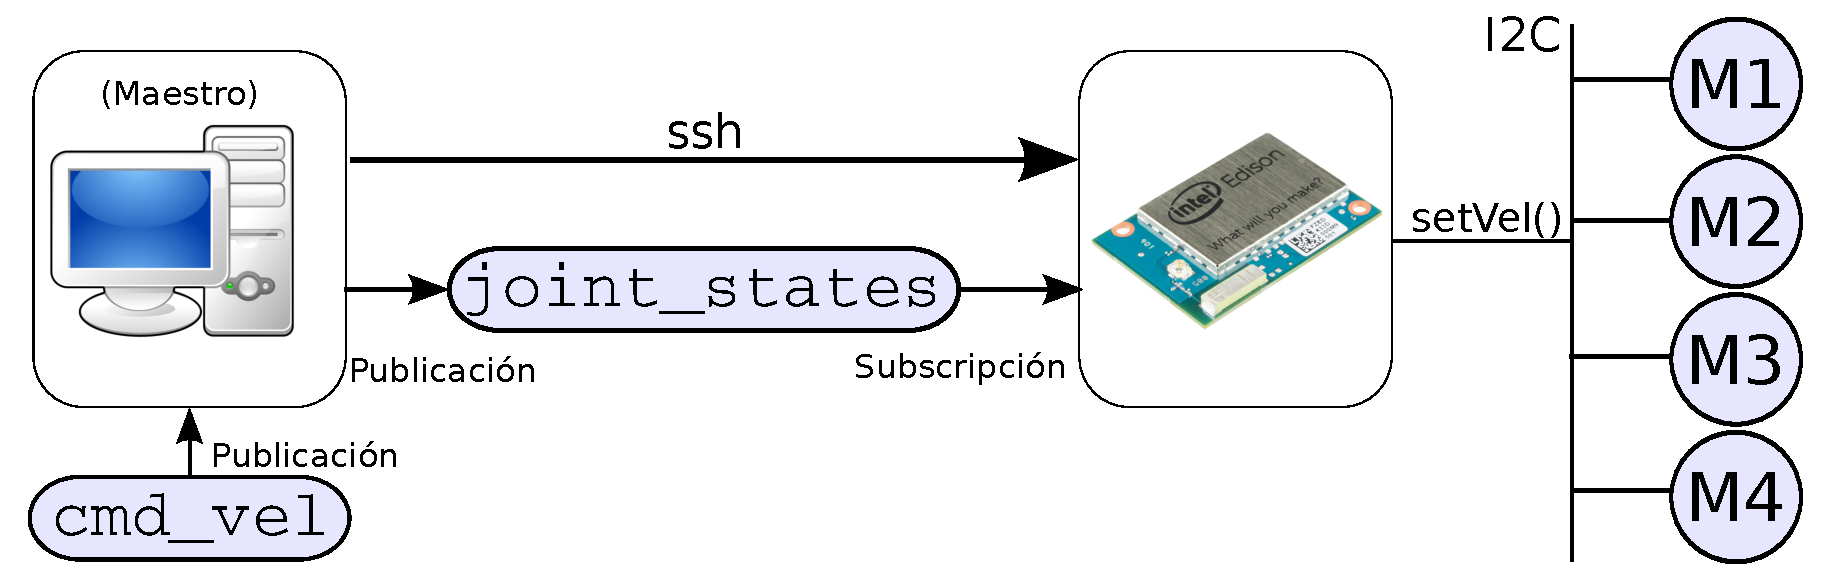
\includegraphics[width = 0.85\linewidth]{imagenes/carro.pdf}
	\end{figure}
\end{frame}

\subsection{Subsección 2}
\begin{frame}
	\frametitle{Título 3}
	\framesubtitle{Título 4}
	\begin{itemize}
		\item Item 1.
		\item Item 2.
		\item Item 3.
	\end{itemize}
\end{frame}

\subsection{Subsección 3}
\subsection{Subsección 4}

\section{Sección 2}
\subsection{Subsección 1}
\begin{frame}
	\frametitle{Título 1}
	\framesubtitle{Título 2}
	\begin{itemize}
		\item Item 1.
		\item Item 2.
		\item Item 3.
	\end{itemize}
	
	\begin{figure}[htb]
		\centering
		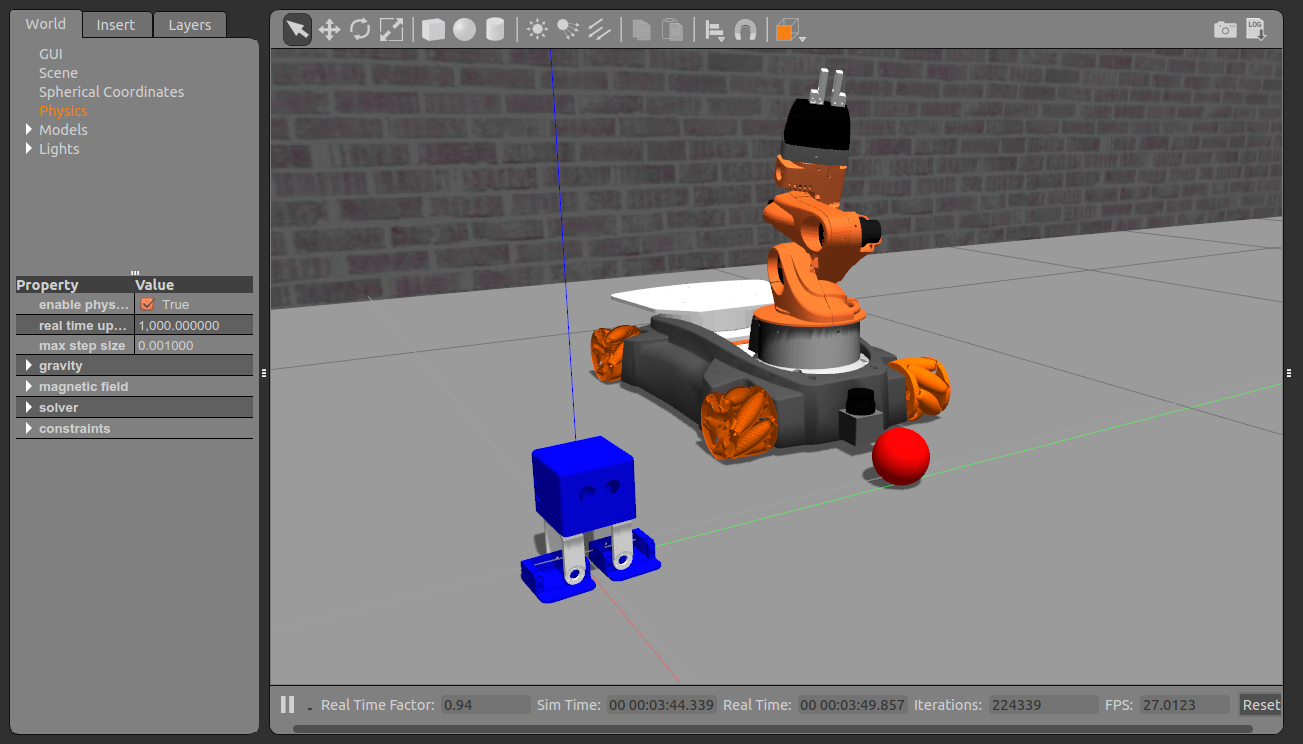
\includegraphics[width = 0.6\linewidth]{imagenes/gaz2.png}
	\end{figure}
\end{frame}

\subsection{Subsección 2}
\begin{frame}
	\frametitle{Título 1}
	\framesubtitle{Título 2}

	\begin{figure}[htb]
		\centering
		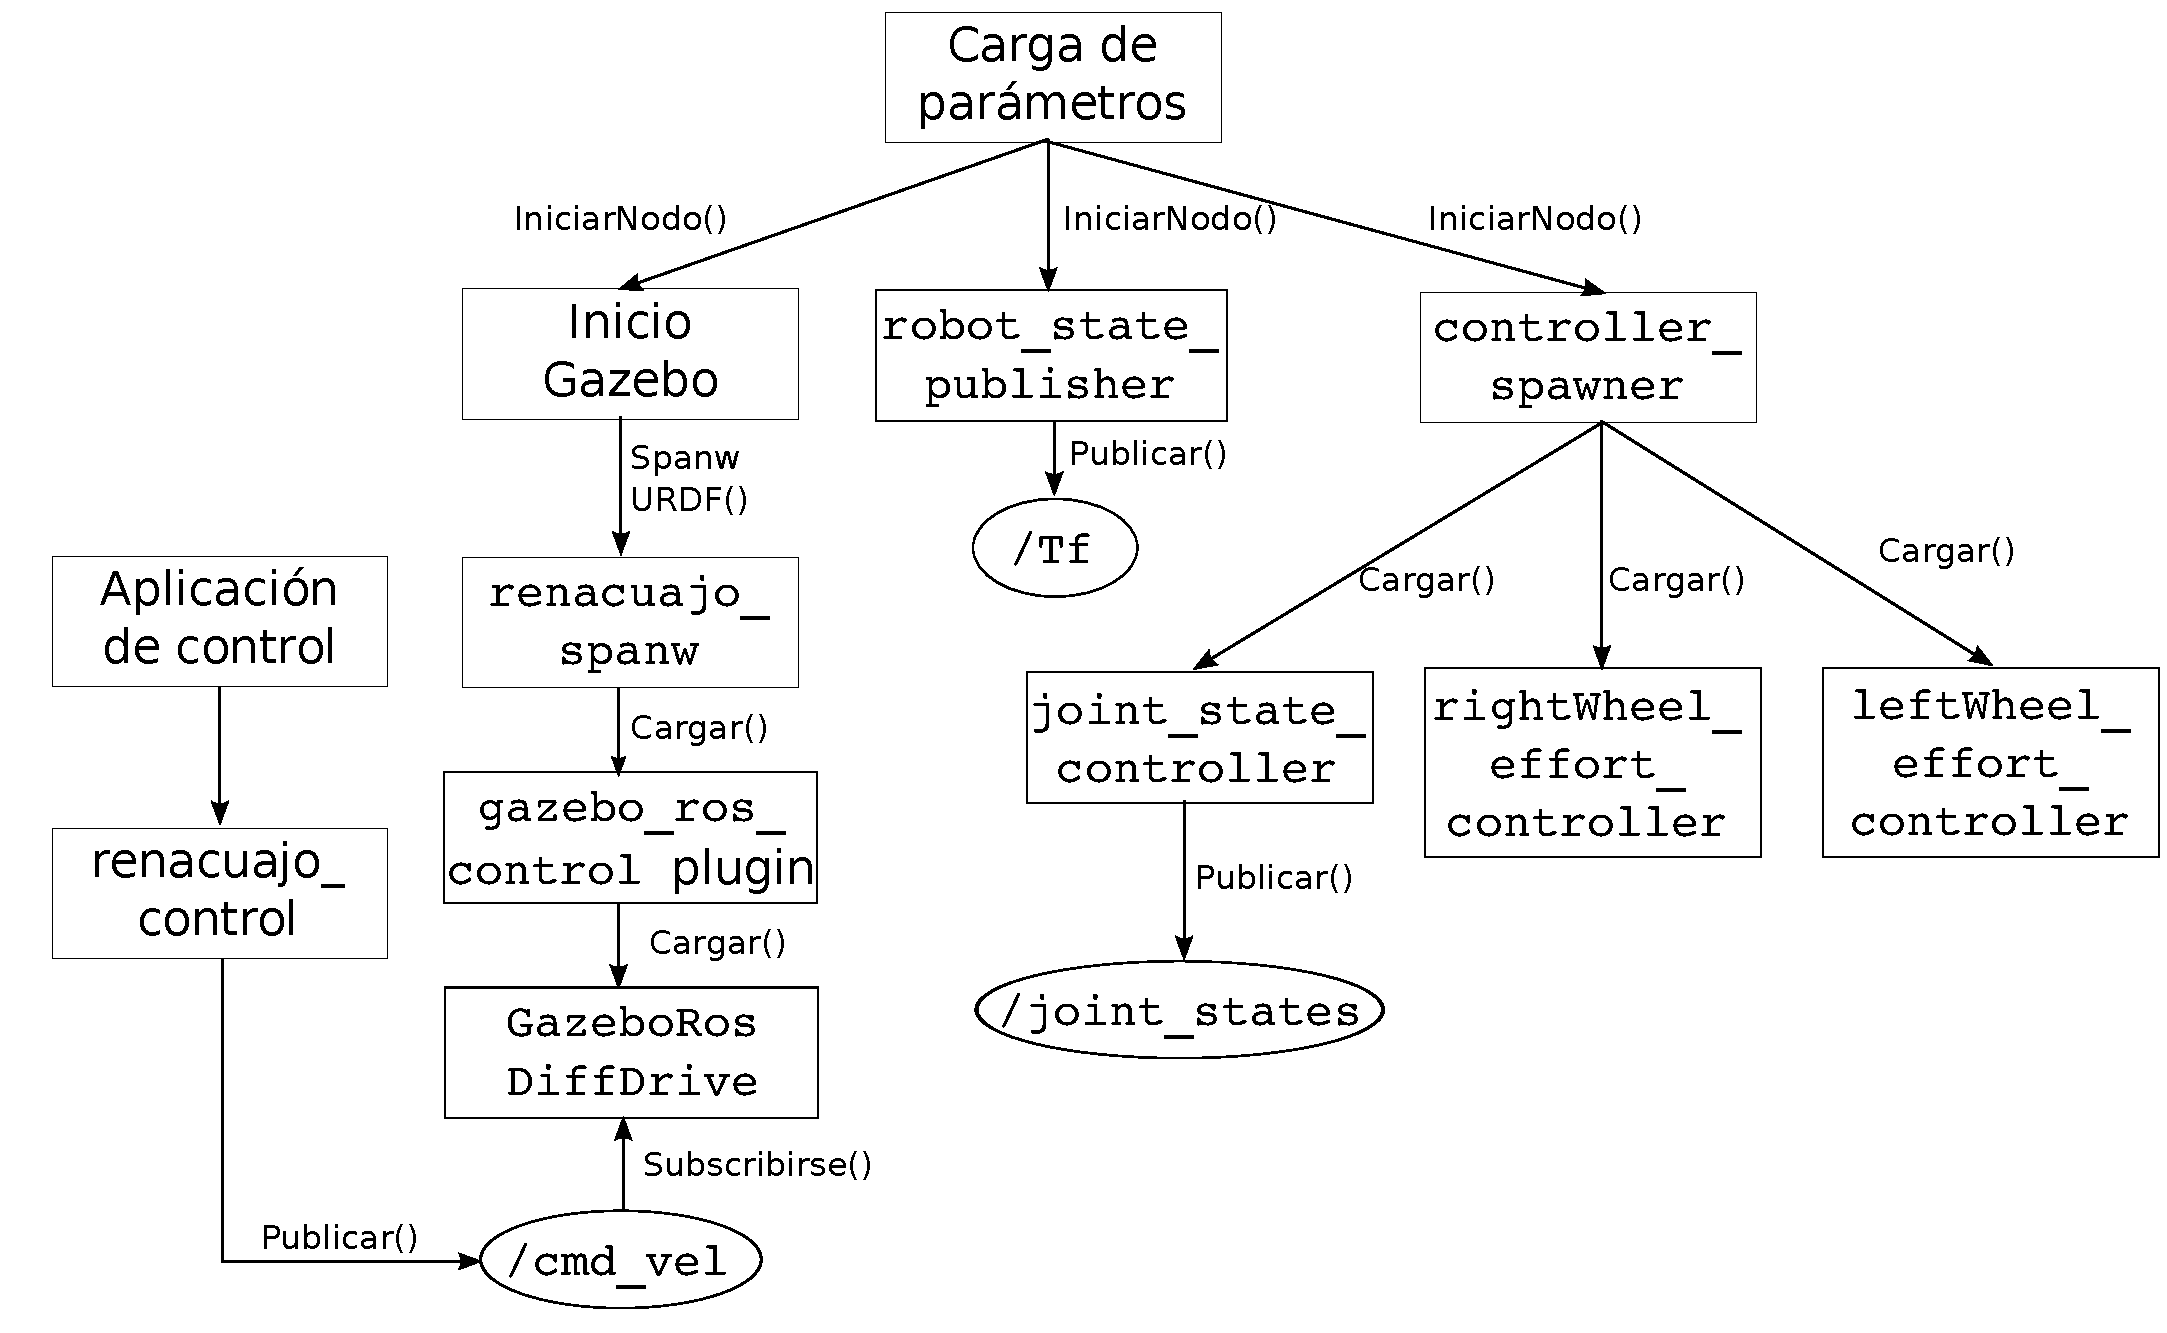
\includegraphics[width = 1\linewidth]{imagenes/sim_renacuajo.pdf}
	\end{figure}
\end{frame}

\section{Sección 3}
\subsection{Subsección 1}
\begin{frame}[fragile]
	\frametitle{Título 1}
	\begin{itemize}
		% Significado URDF
		\item Representar modelos de robots.
		\begin{itemize}
			\item Permite describir las partes mecánicas de un robot y todas sus especificaciones.
		\end{itemize}
	\end{itemize}
	
	\begin{columns}[c]
		\column{.45\textwidth}
		\begin{figure}[htb]
			\centering
			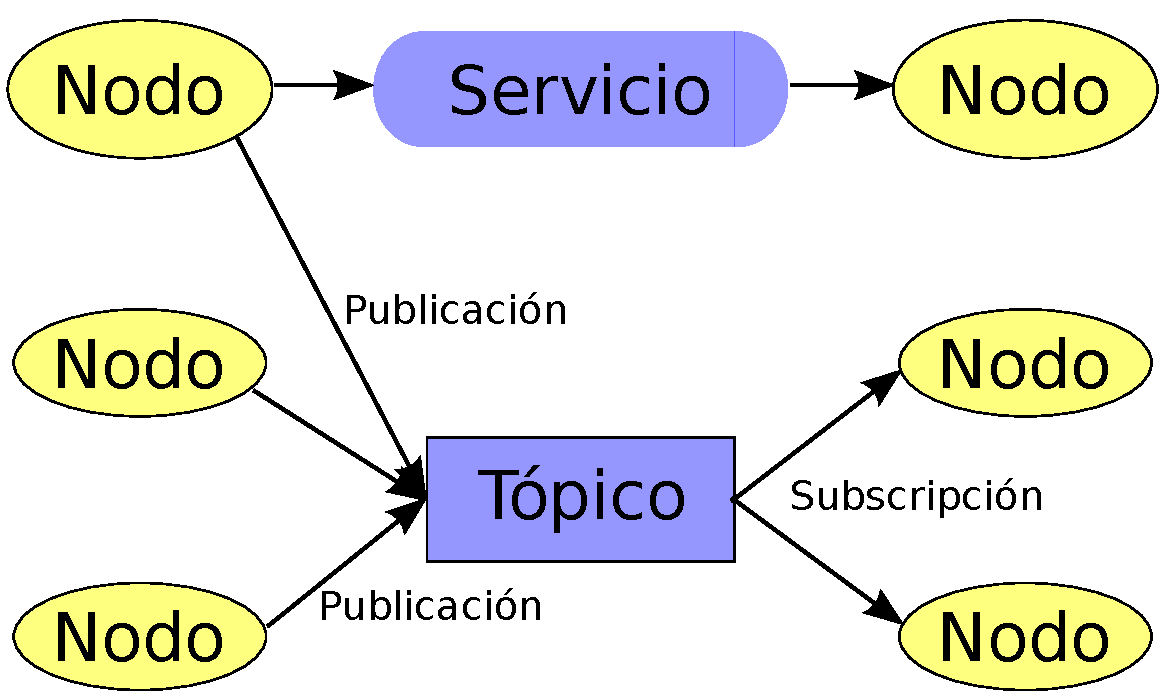
\includegraphics[width = 01\linewidth]{imagenes/estructura_nodos.pdf}
			%\caption{Logo de ROS}
			\label{Figura3_81}
		\end{figure}
		\column{.55\textwidth}
		\begin{block}{URDF}		
			\begin{lstlisting}[language=XML]
			<robot name="robot">
			<link> ... </link>
			<link> ... </link>
			<link> ... </link>
			
			<joint>  ....  </joint>
			<joint>  ....  </joint>
			<joint>  ....  </joint>
			</robot>
			\end{lstlisting}
		\end{block}
	\end{columns}
	
\end{frame}



\subsection{Subsección 2}
\begin{frame}[fragile]
	\frametitle{Generación Automática de URDF}
	
	\begin{columns}[c]
		\column{.35\textwidth}
		\begin{figure}[htb]
			\centering
			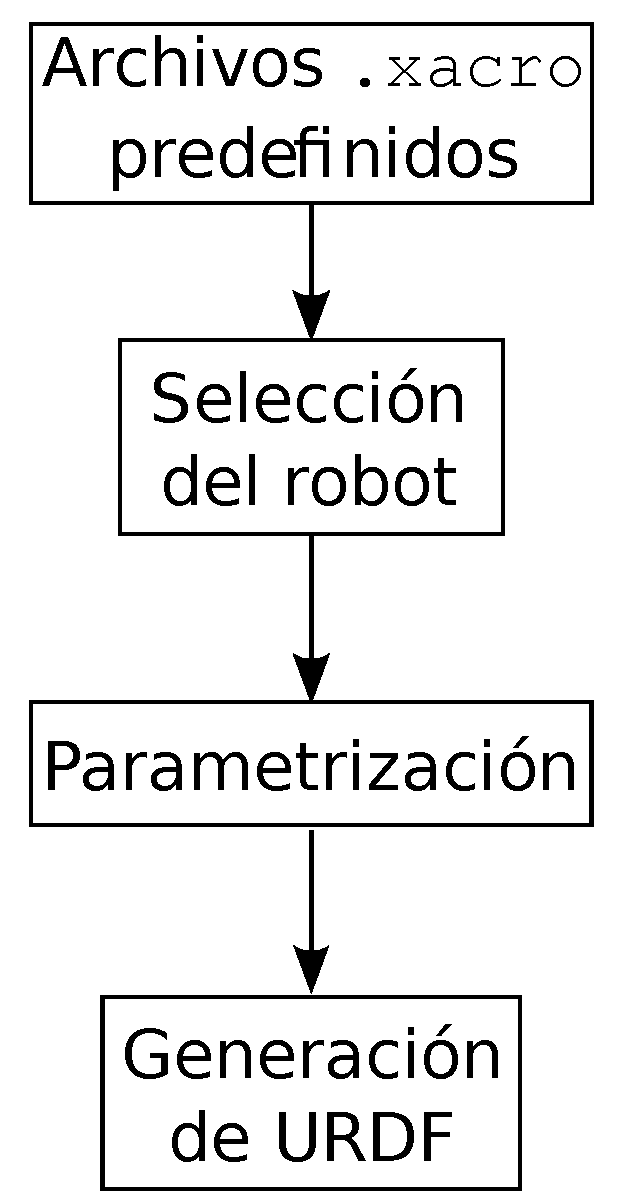
\includegraphics[width = 0.8\linewidth]{imagenes/generacion_automatica.pdf}
		\end{figure}
		\column{.55\textwidth}

			\begin{figure}[htb]
				\centering
				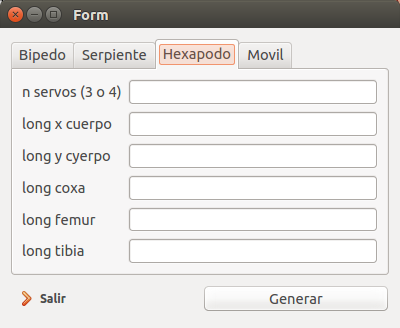
\includegraphics[width = 1\linewidth]{imagenes/generador_urdf.png}
				%\caption{Logo de ROS}
				\label{Figura3_83}
			\end{figure}
	\end{columns}	
\end{frame}

\DiapositivaText{Texto}


\begin{frame}
	\frametitle{Título 1}
	\framesubtitle{Video 1}
	\href{run:videos/ser.avi?autostart&loop}{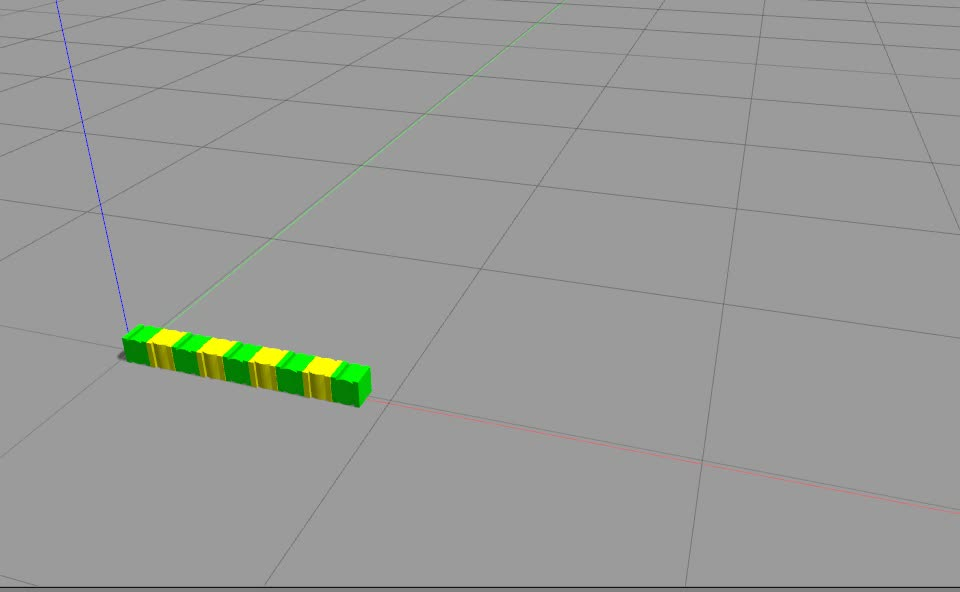
\includegraphics[width=0.8\linewidth,keepaspectratio]{videos/ser.jpg}} 
\end{frame}

\section{Sección 4}
\subsection{Subección 1}
\begin{frame}
	\frametitle{Título 1}
	\framesubtitle{Título 2}
	\begin{itemize}
		\item Item 1.
		\item Item 2.
		\item Item 3.
	\end{itemize}
\end{frame}
\subsection{Subección 2}
\begin{frame}
	\frametitle{Título 1}
	\framesubtitle{Título 2}
	\begin{itemize}
		\item Item 1.
		\item Item 2.
		\item Item 3.
	\end{itemize}
\end{frame}
\subsection{Subección 3}
\DiapositivaText{Texto3}
\subsection{Subección 4}
\begin{frame}
	\frametitle{Título 1}
	\framesubtitle{Título 2}
	\begin{itemize}
		\item Item 1.
		\item Item 2.
		\item Item 3.
	\end{itemize}
\end{frame}

\section{Sección 5}
\subsection{Subección 1}
\ThankYouFrame
\end{document}